\section{实验分析}

为了验证本章所提出的随机Top-$k$算法的性能,我们在4个不同类型数据集上使用不同的模型进行了实验:
\begin{itemize}
    \item CIFAR-100~\cite{krizhevsky_2009_cifar}: 一个常用图像数据集,包含了100类总共5万张大小为$32\times 32$的彩色图片。
        我们使用ResNet-20模型~\cite{hekaiming2016resnet}进行分类,拆分层设置为最后的隐层,大小为128。
    %
    \item YooChoose(1/64)~\cite{ben2015yoochoose,lijing_2017_narm}:RecSys15挑战时公布的YooChoose推荐数据集的按时间顺序划分的1/64子集,包含了大约15万条用户的点击序列,总共有约1.8万个商品类别。
        我们使用GRU4Rec模型~\cite{hidasi_2016_gru4rec}进行分类,隐层大小设置为300。
        拆分层设置为最后的隐层,大小为300。
    %
    \item DBPedia~\cite{2007dbpedia}:一个文本分类数据集,包含了219种类别,总共有大约34万条文本。
        我们采用TextCNN模型~\cite{kimyoon2014textcnn}进行分类,卷积核的大小为 $(3,4,5)$,并且使用Glove预训练词向量~\cite{pennington2014glove}。
        拆分层设置为最后的隐层,大小为300。
    %
    \item Tiny-Imagenet~\cite{tiny-imagenet}:一个图像分类数据集,包含了200类的10万张彩色图片,图片尺寸为$64\times 64$。
        我们采用EfficientNet-b0模型~\cite{tanmingxing2019efficientnet}进行分类。
        拆分层设置为最后的隐层,大小为1280。
        此外,我们对权重采用ImageNet~\cite{2009_imagenet}的预训练权重初始化和随机初始化两种情况分别进行了实验并汇报结果。
\end{itemize}

在每个任务中,我们测试了不同的模型压缩方法和压缩比率,并且对每一个设定都重复了5次实验,报告其平均值。
%
实验的代码基于Pytorch框架~\cite{2019_pytorch}编写,在带有NVIDIA RTX 3090的服务器上进行。
%
实验时我们按照8:1:1的比例划分训练集、验证集合测试集(对于Yoochoose数据集按照时间顺序划分),使用早停(Early Stop)策略获得验证集上最佳的模型,然后在测试集上评估得到准确率。

\begin{table*}[h]
    \centering
    \setlength\tabcolsep{10pt}
    \renewcommand{\arraystretch}{0.8}
    \caption{实验结果:准确率和压缩比率}
    \label{tab:randomized_topk:main-result}
    \small
    \begin{tabular}{@{}ccrrrrr@{}}
    \toprule
    任务          & 压缩  & 随机top-$k$                        & Top-$k$                        & 缩小拆分层             & 量化                 & L1正则化    \\ \midrule
    \multirow{3}{*}{\begin{tabular}[c]{@{}c@{}}CIFAR-100\\      67.20\end{tabular}}\hspace{-3pt}      
        & 高      & \textbf{65.25 / 2.86}       & \underline{62.23 / 2.86} & 55.52 / 3.13       & -                            & -          \\ \cmidrule(lr){2-7} 
        & 中      & \textbf{65.83 / 5.71}       & \underline{61.56 / 5.71} & 60.43 / 6.25       & 53.56 / 6.25          & \underline{62.11 / 8.41}   \\ \cmidrule(lr){2-7} 
        & 低      & \underline{65.98 / 12.4}         & 62.11 / 12.3       & 62.93 / 12.4       & \textbf{66.01 / 12.5} & 63.87 / 19.5          \\ \midrule
    \multirow{3}{*}{\begin{tabular}[c]{@{}c@{}}YooChoose\\      63.57\end{tabular}}\hspace{-3pt}      
        & 高      & \textbf{60.29 / 0.85}       & \underline{60.28 / 0.85} & 50.71 / 1.00       & -                            & -          \\ \cmidrule(lr){2-7} 
        & 中      & \textbf{64.55 / 1.71}       & \underline{63.81 / 1.71} & 62.20 / 2.00       & -                            & -                                   \\ \cmidrule(lr){2-7} 
        & 低      & \textbf{66.88 / 3.84}       & \underline{66.12 / 3.84} & \underline{66.12 / 4.00} & 64.69 / 3.13          & 61.48 / 3.01          \\ \midrule
    \multirow{4}{*}{\begin{tabular}[c]{@{}c@{}}DBPedia\\      93.11\end{tabular}}\hspace{-3pt}        
        & 很高    & \textbf{84.88 / 0.44}       & \underline{83.04 / 0.44} & 64.80 / 0.50       & -                            & -          \\ \cmidrule(lr){2-7} 
        & 高      & \textbf{88.01 / 0.88}       & \underline{85.49 / 0.88} & 78.57 / 1.00       & -                            & 81.35 / 1.08          \\ \cmidrule(lr){2-7} 
        & 中      & \textbf{90.50 / 1.97}       & 87.74 / 1.97       & 86.42 / 2.00       & -                            & \underline{87.88 / 0.93}    \\ \cmidrule(lr){2-7} 
        & 低      & \underline{91.59 / 3.06}          & 90.05 / 3.06       & 88.38 / 3.00       & 91.20 / 6.25          & \textbf{93.11 / 5.31} \\ \midrule
    \multirow{3}{*}{\begin{tabular}[c]{@{}c@{}}Tiny-ImageNet \\ 随机初始化 \\      53.11\end{tabular}}\hspace{-3pt}   
        & 高      & \textbf{50.83 / 0.21}       & 48.36 / 0.21       & 35.46 / 0.23       & -                            & -           \\ \cmidrule(lr){2-7} 
        & 中      & \textbf{51.75 / 0.42}       & \underline{47.24 / 0.42} & 45.66 / 0.47       & -                            &  -                                 \\ \cmidrule(lr){2-7} 
        & 低      & \textbf{51.16 / 0.94}       & 45.50 / 0.94       & \underline{48.87 / 0.14} & -                            & -                                   \\ \midrule
    \multirow{3}{*}{\begin{tabular}[c]{@{}c@{}}Tiny-ImageNet \\ 预训练 \\ 75.18\end{tabular}}\hspace{-3pt} 
        & 高      & \textbf{71.09 / 0.21}       & \underline{70.86 / 0.21} & 59.23 / 0.23       & -                            & -           \\ \cmidrule(lr){2-7} 
        & 中      & \textbf{72.15 / 0.42}       & \underline{71.19 / 0.42} & 66.52 / 0.47       & -                            & -                                   \\ \cmidrule(lr){2-7} 
        & 低      & \textbf{73.83 / 0.94}       & \underline{72.52 / 0.94} & 68.67 / 0.94       & -                            & 67.82 / 1.24          \\ \bottomrule
    \end{tabular}
\end{table*}


\subsection{压缩比率和模型准确率对比}
%
我们评估了模型在测试集上的准确率(对于Yoochoose数据集,我们用前20准确率代替)。
%
我们在CIFAR-100, DBPedia, Tiny-Imagenet三个任务上把随机Top-$k$的随机参数$\alpha$设置为0.1,在Yoochoose任务上设置为0.05。
%
我们把实验结果汇报在\autoref{tab:randomized_topk:main-result}中。
表内每一项的格式为“准确率/压缩比率(\%)”,任务名称下方的准确率表示无压缩的普通拆分学习的准确率(压缩比率=100)。
表内空白项表示该方法在本文的实验中无法达到对应的压缩比率。
我们用粗体表示同等压缩比率下最高的准确率,用下划线表示次高的准确率。


实验结果表明,随机Top-$k$算法几乎在所有任务上都取得了最好的准确率和最低的压缩比率,且大幅领先于其他方法,在很低的压缩比率情况下依然保持了和原始无压缩拆分学习相近的表现。
%
在YooChoose任务中,随机Top-$k$算法甚至超过了无压缩的拆分学习,我们认为这可能归功于随机Top-$k$的正则化效果抑制了过拟合现象。
%
同时,我们注意到,量化方法和L1正则化方法难以达到一些较低的压缩比率。
这是因为在原始模型采用常用的32位浮点数计算时,量化方法最低只能达到1/32的压缩比率,并且此时拆分层表征被压缩为二值,往往会导致模型训练无法收敛。
而L1正则化在系数过大时也会导致模型无法收敛,而且通过正则化系数并不能直接控制稀疏程度,同一个正则化系数也可能训练得到稀疏程度不同的模型。
%

\subsection{训练速度分析}
\begin{figure}[h!]
    \centering
    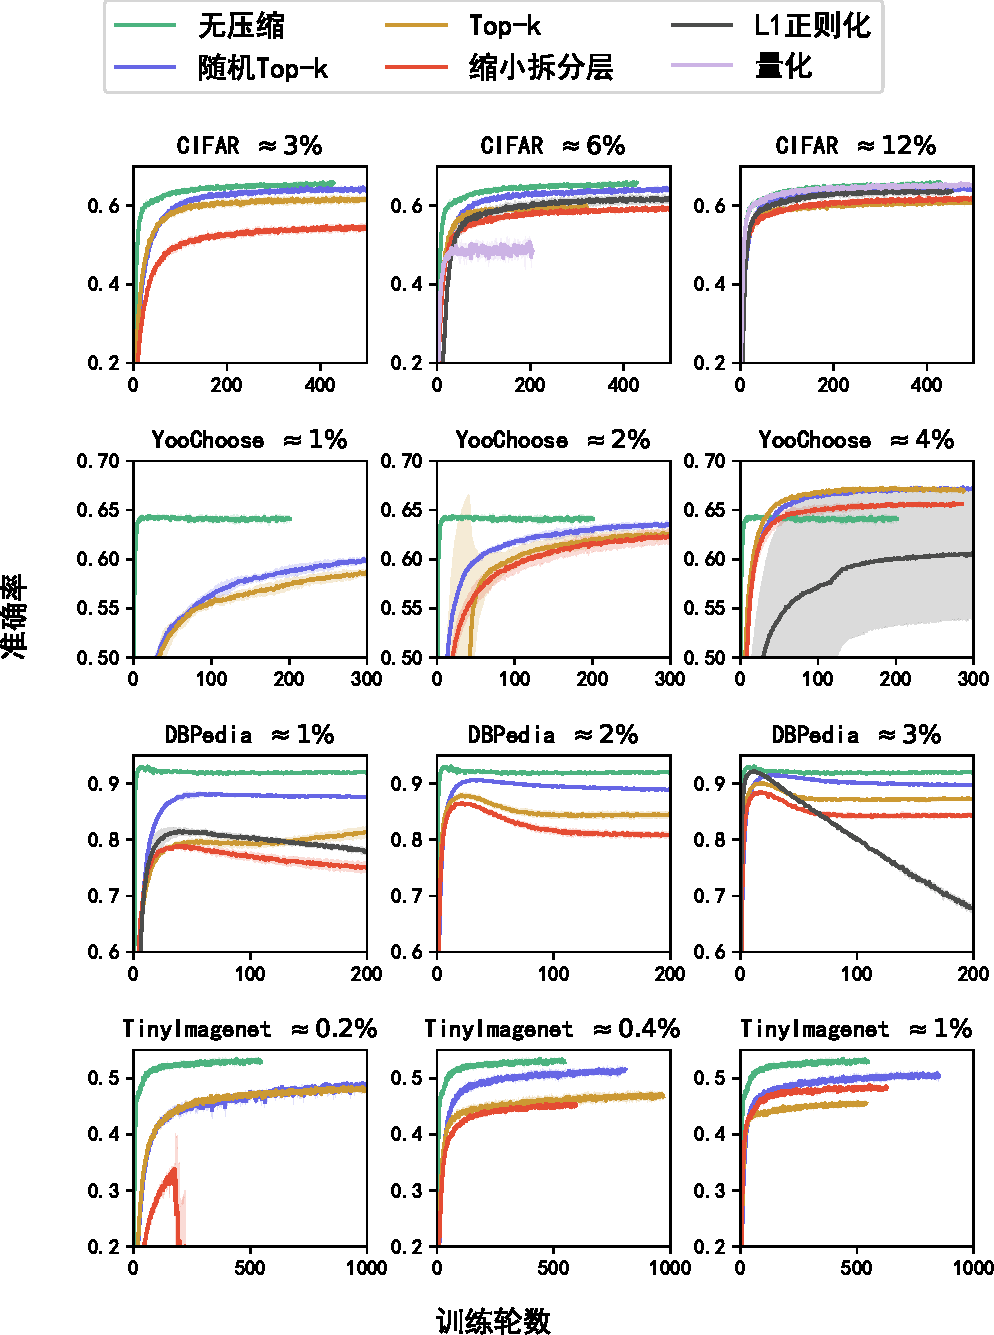
\includegraphics[width=1\linewidth]{Z_Resources/randtopk_acc-epoch}
    \caption{不同压缩方法的训练轮次和准确率曲线图}
    \label{fig:randomized_topk:training-epoch}
\end{figure}

\begin{figure}[h!]
    \centering
    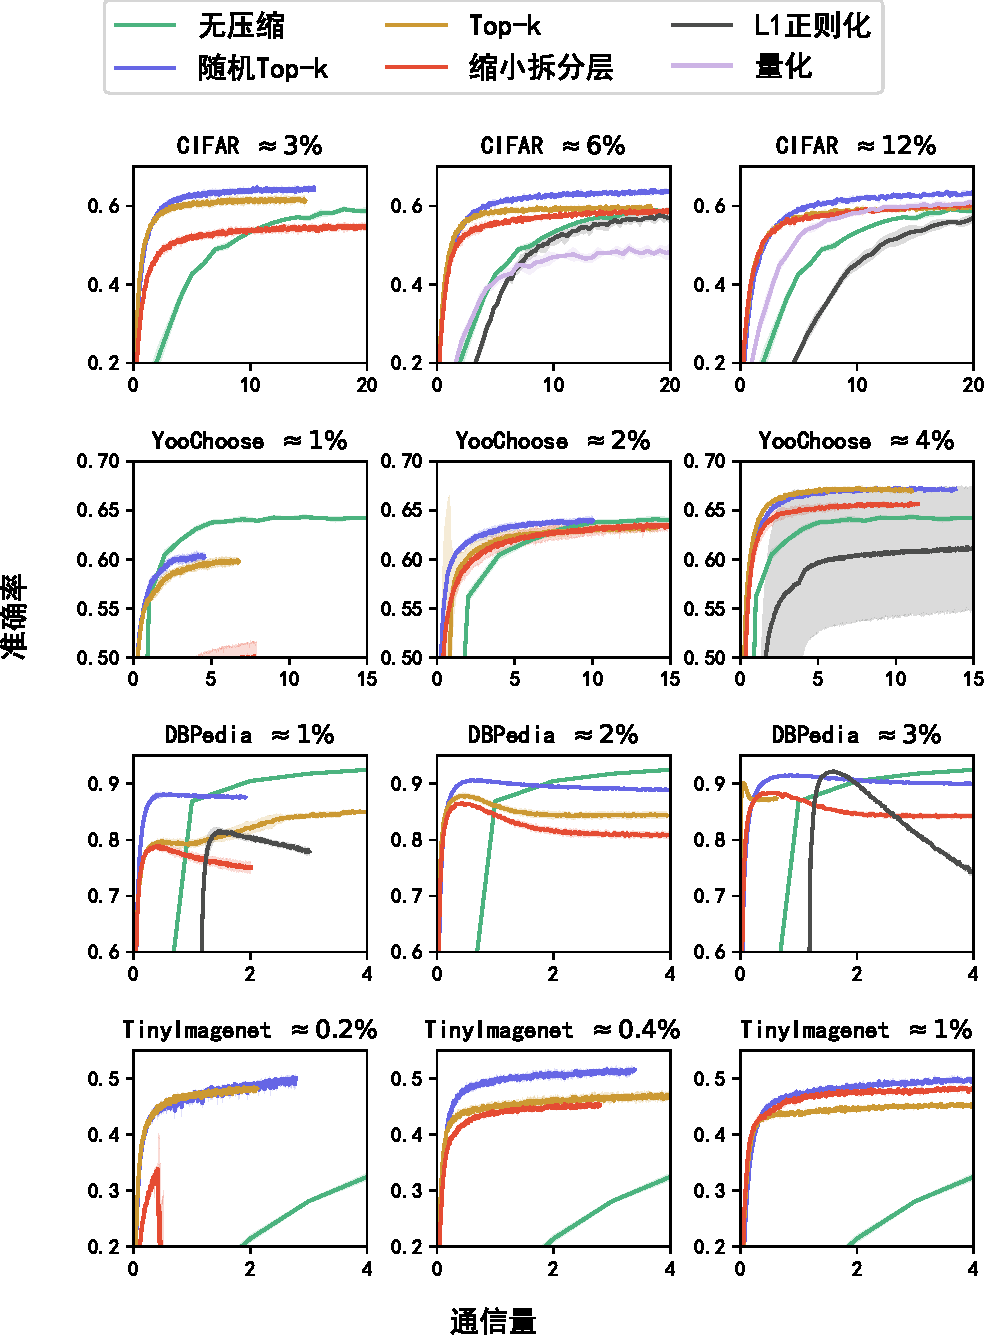
\includegraphics[width=1\linewidth]{Z_Resources/randtopk_acc-comm}
    \caption{不同压缩方法的通信量和准确率曲线图}
    \label{fig:randomized_topk:training-comm}
\end{figure}


我们在\autoref{fig:randomized_topk:training-epoch}和\autoref{fig:randomized_topk:training-comm}中分别汇报了训练过程中准确率和训练轮次以及通信量的关系。
压缩比率被标识在每个曲线图上方。
%
我们将未压缩的一轮训练通信量设置为1。
%
实验结果表明,无压缩的拆分学习收敛所需要的训练轮次数最少。
尽管如此,其他压缩方法依然可以在几十轮内收敛到较高的准确率,且随机Top-$k$的收敛速度相对领先。
%
以训练所需的通信量衡量时,几乎所有压缩方法的收敛所消耗的通信量都显著低于无压缩的拆分学习,并且相比于其他方法,随机Top-$k$的收敛速度和准确率都是最高的。
%
而L1正则化以及量化算法在反向传播时需要传播所有的梯度以确保训练效果,只能压缩前向传播的表征,因此其训练时通信量的降低幅度必然小于50\%,导致了较大的通信开销。
%
也可以注意到L1正则化的训练不稳定,有较高的误差范围,这是因为为了达到高压缩率,我们需要选取较大的L1正则化系数,影响了损失函数的收敛。
%

\subsection{随机参数$\alpha$分析}
本节我们报告了选取不同随机参数$\alpha$时的实验结果,包括了$\alpha$和准确率、收敛速度、泛化误差、Top-$k$神经元分布、以及输入特征重构攻击效果的关系,为选取合适的$\alpha$提供参考,并且验证前文关于收敛性、泛化效果以及隐私保护的理论分析。


\begin{figure}[h!]
    \centering
    \begin{subfigure}{0.46\linewidth}
        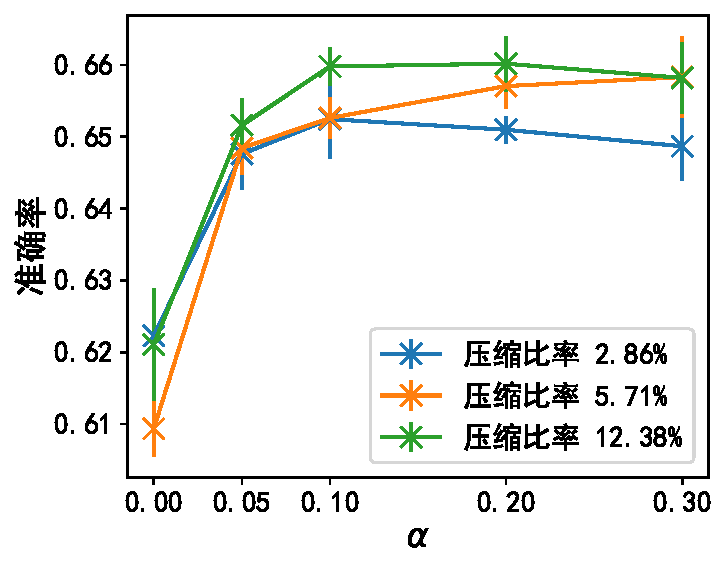
\includegraphics[width=1\linewidth]{Z_Resources/随机topk_cifar-alpha.pdf}
        \subcaption{CIFAR}
        \label{fig:cifar-trainloss}
    \end{subfigure}
    \begin{subfigure}{0.46\linewidth}
        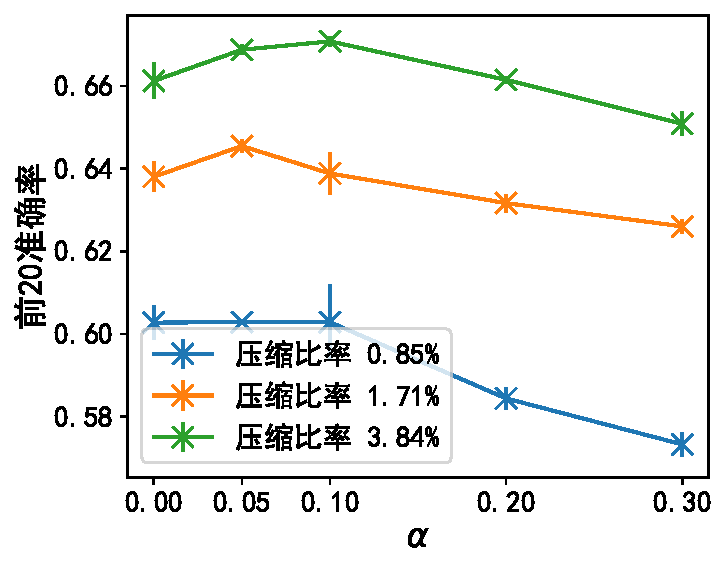
\includegraphics[width=1\linewidth]{Z_Resources/随机topk_yoochoose-alpha.pdf}
        \subcaption{YooChoose}
        \label{fig:cifar-generror}
    \end{subfigure}
    \caption{$\alpha$与准确率的关系}
    \label{fig:randomized_topk-alpha-acc}
\end{figure}

\begin{figure}[h!]
    \centering
    \begin{subfigure}{0.45\linewidth}
        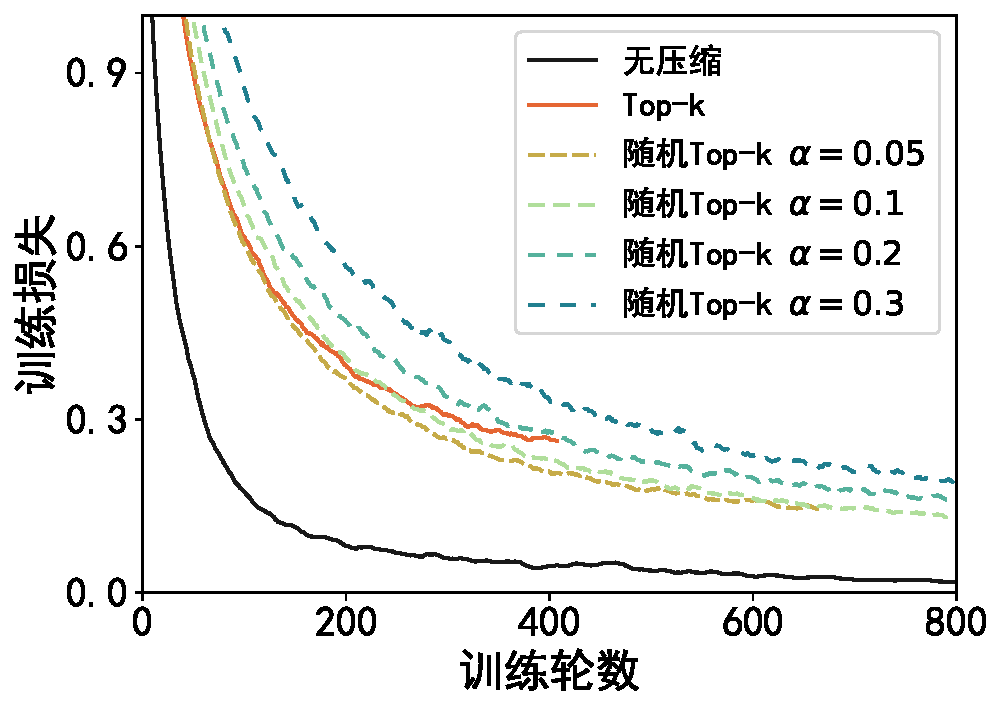
\includegraphics[width=1\linewidth]{Z_Resources/randtopk_cifar100-trainacc.pdf}
        \subcaption{训练损失}
        \label{fig:randomized_topk-cifar-trainloss}
    \end{subfigure}
    \begin{subfigure}{0.47\linewidth}
        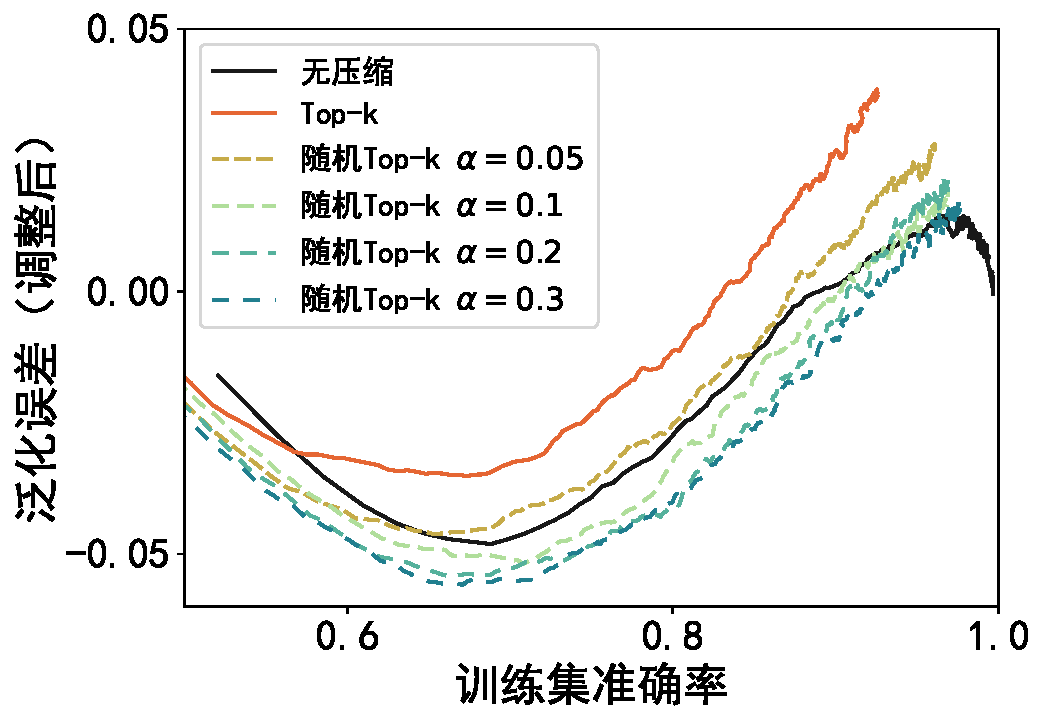
\includegraphics[width=1\linewidth]{Z_Resources/randtopk_cifar100-generror.pdf}
        \subcaption{泛化误差}
        \label{fig:randomized_topk-cifar-generror}
    \end{subfigure}
    \caption{$\alpha$与训练损失以及泛化误差的关系}
    \label{fig:randomized_topk-alpha-loss}
\end{figure}


\textbf{准确率}:
\autoref{fig:randomized_topk-alpha-acc}展示了在CIFAR-100和YooChoose任务中$k=3$情况下,随机参数$\alpha$与模型测试准确率的关系;
可以看出,在CIFAR-100任务中,无论怎样选取$\alpha$都可以比无压缩情况下显著提高准确率,而在YooChoose任务中,提高的幅度则相对有限。
同时,在$\alpha$ 提高到 0.1之后,准确率随着$\alpha$的进一步提高呈现出下降趋势。
%
分析表明,$\alpha \in [0.5, 1]$ 可以使得模型达到较高准确率;而过大的$\alpha$会引入过多的噪声,从而损害模型的效果。


\textbf{收敛性和泛化误差}:
\autoref{fig:randomized_topk-alpha-loss}展示了在CIFAR-100任务中$k=3$情况下,随机参数$\alpha$与模型训练损失和泛化误差的关系。
为了更清晰呈现泛化误差的变化,我们对泛化误差进行了调整,将\autoref{fig:randomized_topk-cifar-generror}调整为的Y轴调整为如下:
\begin{equation}
    y = \text{泛化误差(训练集准确率 - 测试集准确率)} - 0.5 \times \text{训练集准确率} + 0.2.
\end{equation}
%
从图中可以看出,Top-$k$稀疏化在训练开始时损失下降较快,但是随着训练轮数的增长,随机Top-$k$的损失下降变快,并且最终收敛的损失低于Top-$k$。
另外,太大的$\alpha$也导致损失下降变慢。
%
同时,相对于无压缩的情况,Top-$k$稀疏化显著增加了泛化误差。而增大$\alpha$也显著降低了泛化误差。
%
这和我们在\autoref{sec:randomized_topk:method}中对于随机Top-$k$算法的收敛性和泛化性的理论分析相对应。



\begin{figure}[h!]
    \centering
    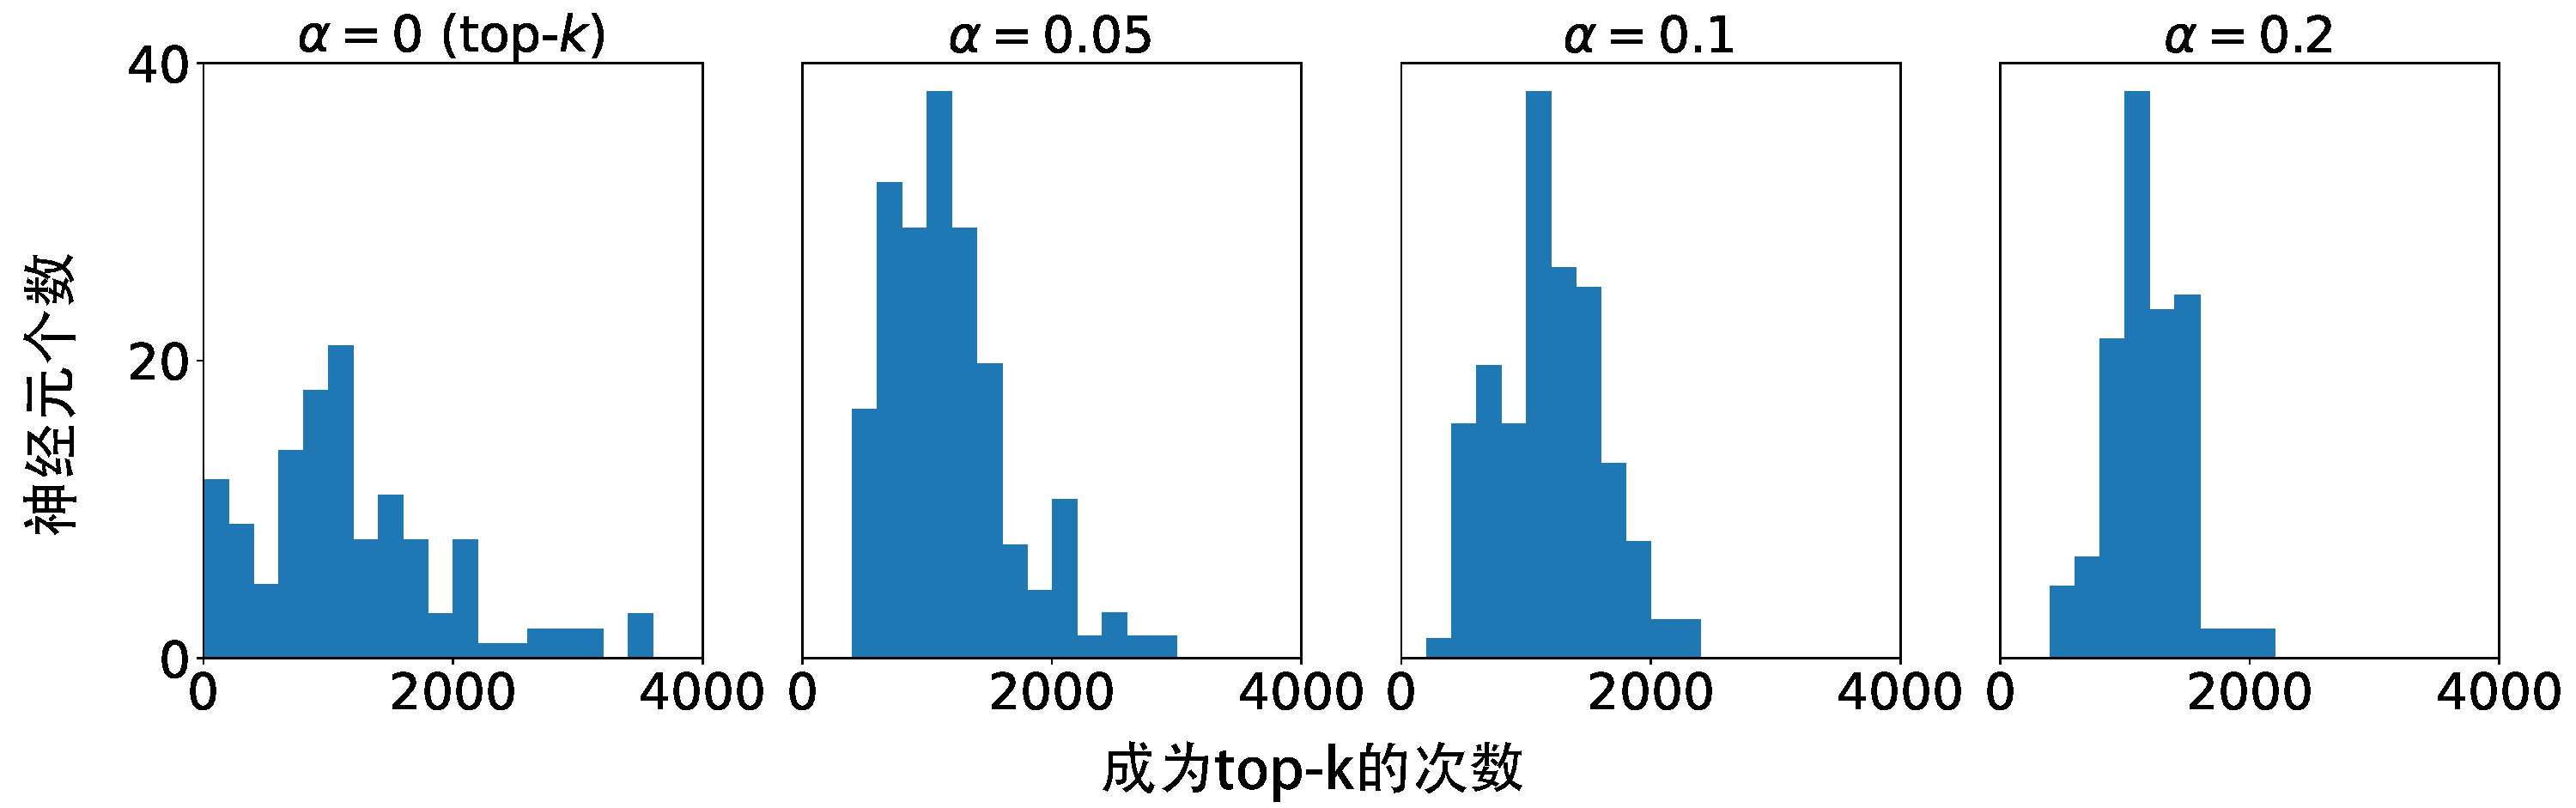
\includegraphics[width=\linewidth]{Z_Resources/随机topk_cifar100-dist-topk.pdf}
    \caption{两方拆分学习推断示意图}
    \label{fig:randomized_topk-dist}
\end{figure}

\textbf{Top-$k$神经元的分布:}
\autoref{fig:randomized_topk-dist}显示了采用不同的$\alpha$训练后,在推断阶段使用测试集样本时,神经元被选为Top-$k$次数的分布。具体而言,隐层的第$i$个神经元被选为Top-$k$的次数按照如下公式计算:
\begin{equation}
    C_i = \sum_{j=1}^N [\text{$M_b(X_j)$的 Top-$k$ 神经元包含了其第 $i$ 个神经元(是=1,否=0)}],
\end{equation}
其中,$N$表示测试集样本数,$X_j$表示第$j$个样本。
%
%
可以看出,仅使用Top-$k$稀疏化时,神经元被选为Top-$k$次数的分布不均匀,部分神经元几乎从未被选为Top-$k$,而某些神经元则总是被选中;而使用随机Top-$k$算法有效地解决了这一问题,Top-$k$次数的分布变得均匀,说明各个神经元被选为Top-$k$的概率更加均等。
%
即使是一个较小的$\alpha$(如0.05),也能显著使得Top-$k$次数的分布变得均匀。
%
这也说明,随机Top-$k$更好地利用了表征空间,从而提高了泛化性能。
%


\begin{figure}[htbp]
    \centering
    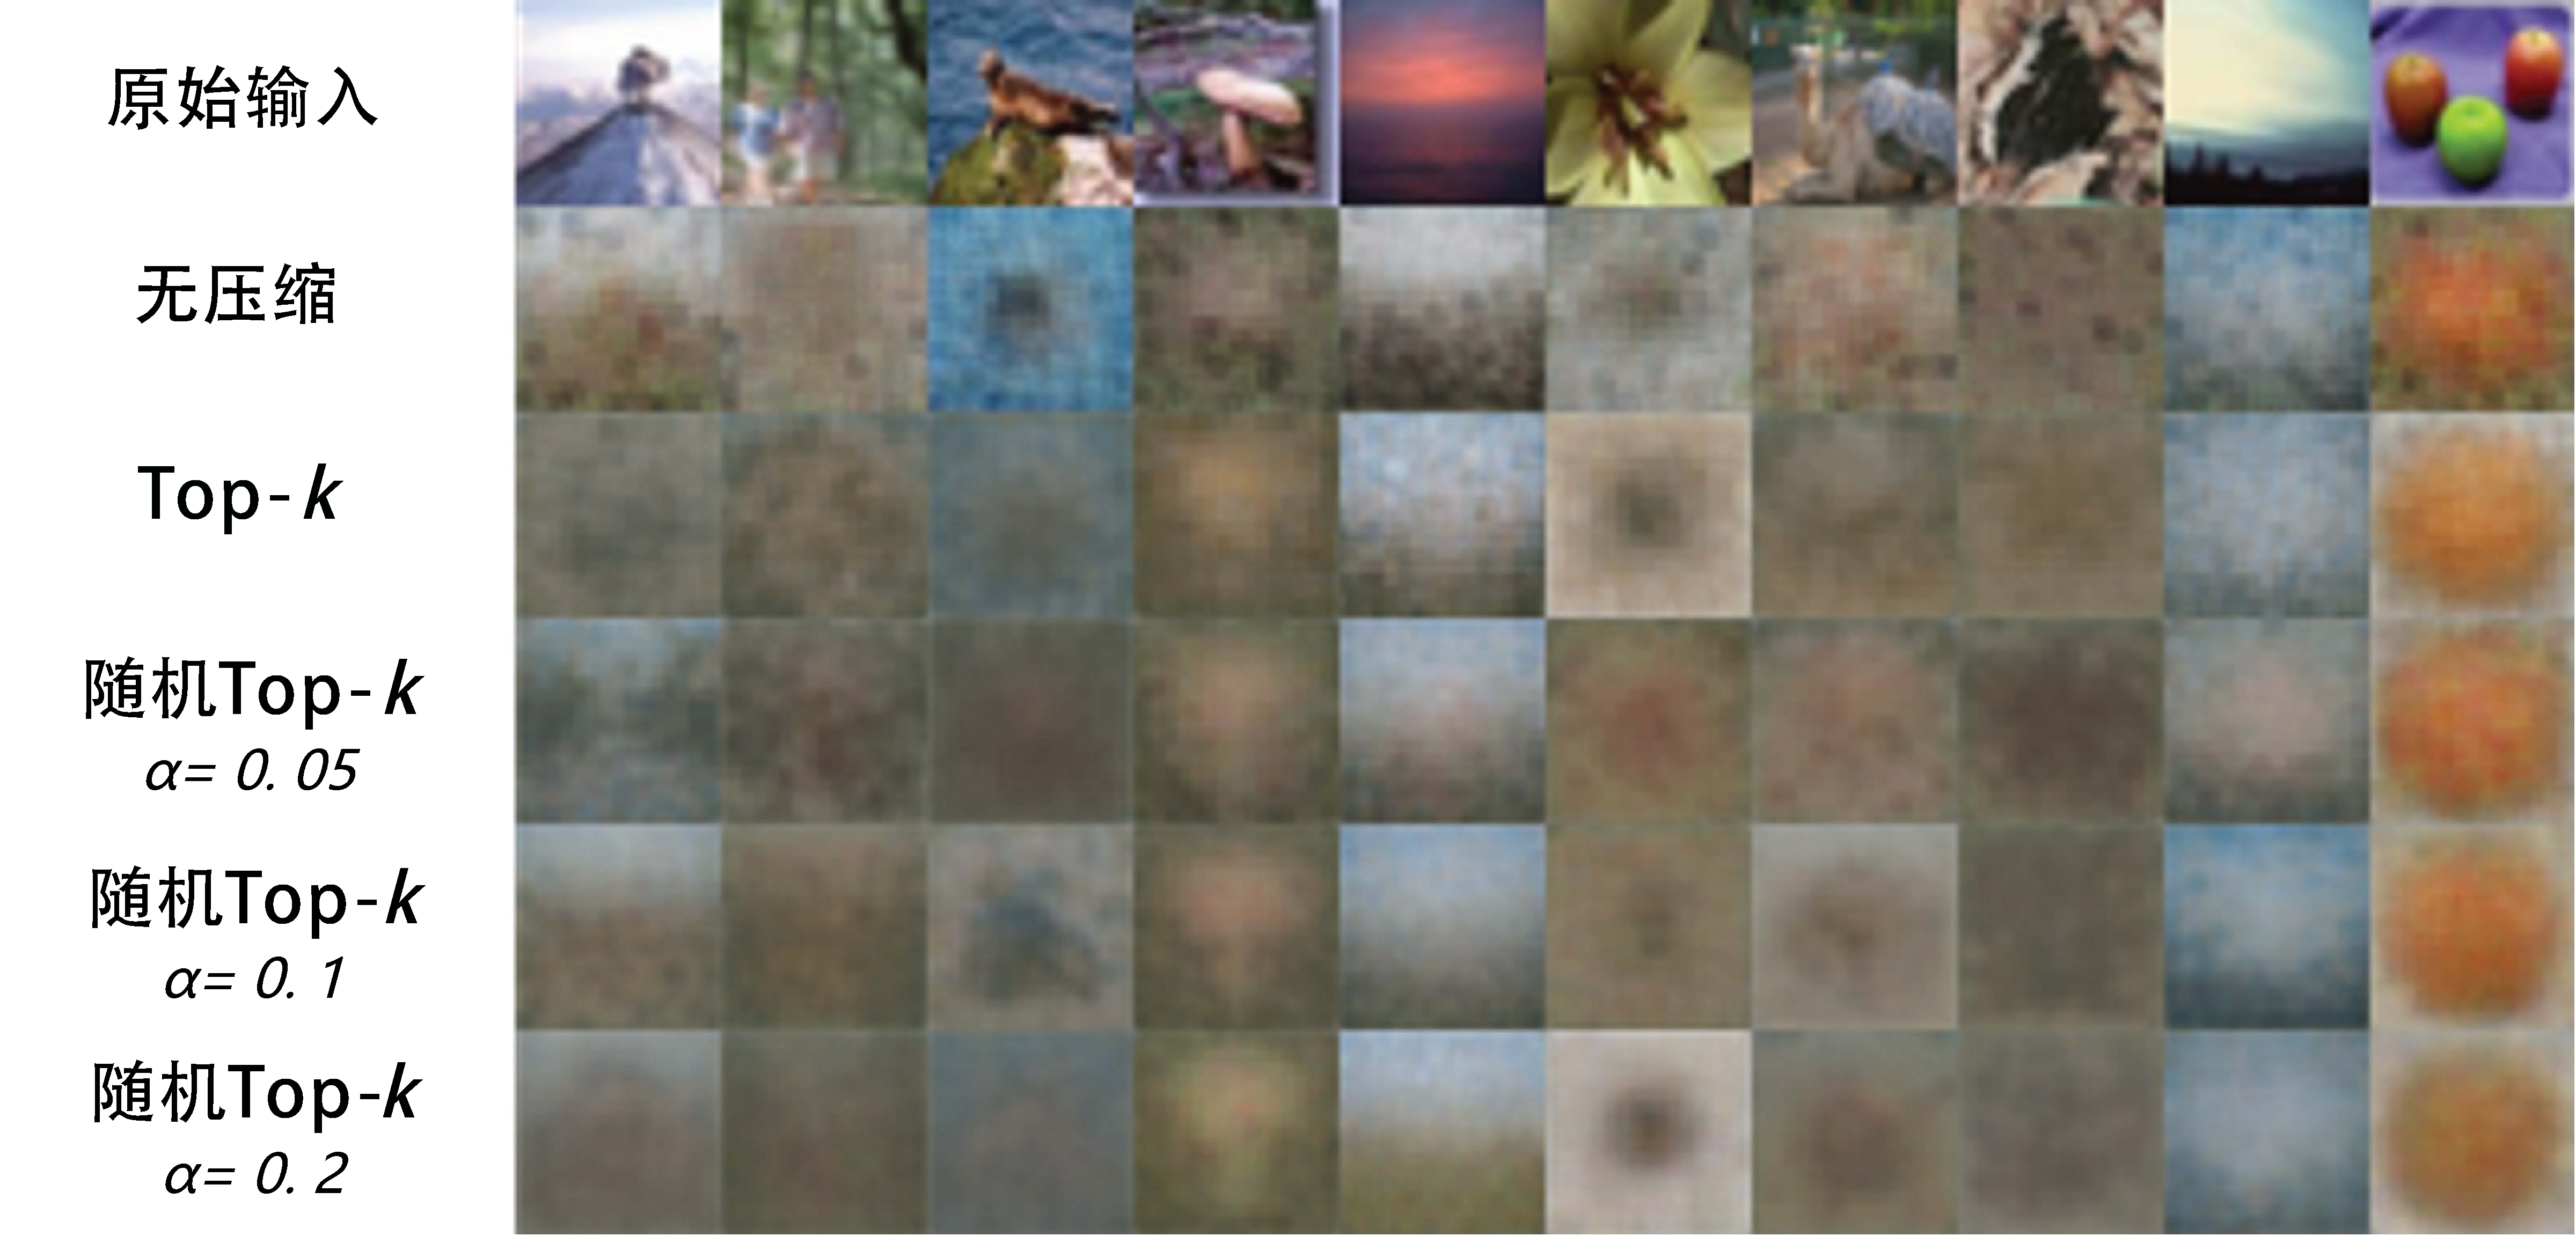
\includegraphics[width=\linewidth]{Z_Resources/随机topk_inversion-attack.pdf}
    \caption{CIFAR-100输入重建攻击效果}
    \label{fig:randomized_topk-inversion_attack}
\end{figure}

\begin{figure}[h!]
    \centering
    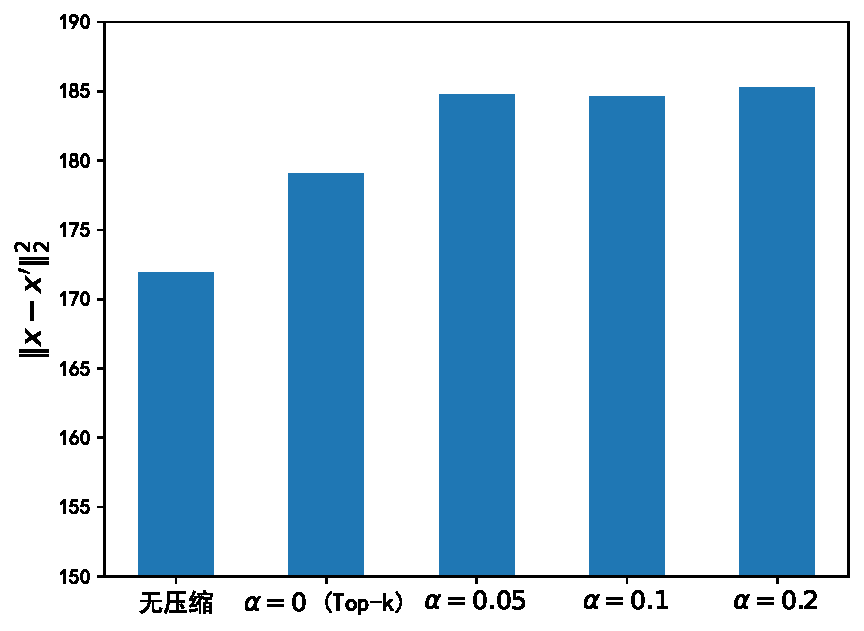
\includegraphics[width=0.58\linewidth]{Z_Resources/randtopk_cifar-attack-error.pdf}
    \caption{CIFAR-100输入重建攻击误差}
    \label{fig:randomized_topk-attack-error}
\end{figure}


\subsection{隐私分析}
为了表明随机Top-$k$压缩方法对于输入数据的隐私的影响,我们在CIFAR-100数据集上进行了输入特征重建攻击的实验。
%
输入重建攻击是一种从隐层恢复出输入数据的手段,其方法是通过泄漏的数据,训练一个重构神经网络将拆分层数据逆向回原始输入特征~\cite{hezecheng_2019_model_inversion_attack,vepakomma2020nopeek}。
%
本实验中,重构神经网络的结构为(全连接,卷积,反卷积,卷积),其中全连接层将128维拆分层投影为$4 \times 16\times 16$ (4表示通道数),此后三层的输出大小分别为$16\times 16 \times  16$,$32\times 32 \times 32$,$3\times 32 \times 32$。激活函数为LeakyReLU~\cite{maas2013leaky_relu}。

\autoref{fig:randomized_topk-inversion_attack}展示了在CIFAR-100任务中$k=3$情况下,在模型推断阶段,攻击者根据拆分层表征对原始输入图片进行恢复攻击的效果。
从图中可以看出,由于拆分层被设置在最后一层线性层,因此即使是无压缩的情况下,攻击者依然难以还原图片的主要信息,只能呈现出模糊的类似于类别的“平均图”的图片。
%
而Top-$k$稀疏化和随机Top-$k$算法进一步使得原始图片中的色彩信息几乎也被丢失。
%

为了更加清晰地显示随机Top-$k$算法和其他方法的输入特征隐私保护效果,我们测量了图片恢复攻击的平方误差,即$\mathbb E\left[ \Vert \text{恢复值} - \text{原始值} \Vert^2 \right]$,并汇报在\autoref{fig:randomized_topk-attack-error}中。
%
从图中可以看出,Top-$k$稀疏化相对于原始无压缩的拆分学习显著提高了攻击者的重建损失,增强了隐私保护效果。
而随机Top-$k$算法比Top-$k$拥有更高的重建损失,说明其进一步提高了对于输入特征的隐私保护。


